%\documentclass{article}
%\usepackage{tikz}
%\begin{document}

\begin{figure}[tb]
	\centering
	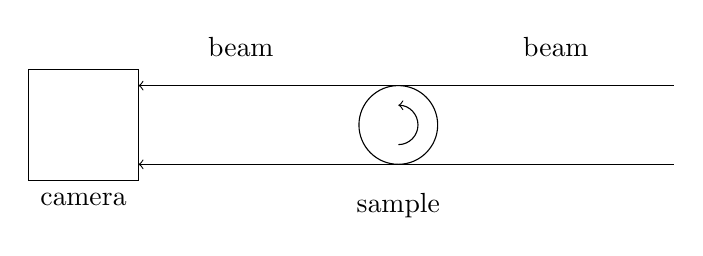
\begin{tikzpicture}
		%drawing grid
		%\draw[color=gray] (0,0) grid (8,1);
		%camera
		\draw (-.2,-.2) rectangle (1.2,1.2);
		\draw (.5,-.25) node [below] {camera};
		% beam
		\draw[<-] (1.2,0) -- (8,0);
		\draw[<-] (1.2,1) -- (8,1);
		\draw (2.5,1.25) node [above] {beam};
		\draw (6.5,1.25) node [above] {beam};
		%sample
		\draw (4.5,0.5) circle (.5);
		\draw (4.5,-.25) node [below] {sample};
		%sample rotation
		\draw[->] (4.5,0.25) arc (-90:90:.25);
	\end{tikzpicture}
	\caption{Covering the FOV -- one scan}
	\label{fig:covering-one scan}
\end{figure}

%\end{document}